\documentclass{exam}

\usepackage{units} 
\usepackage{xfrac} 
\usepackage[fleqn]{amsmath}
\usepackage{cancel}
\usepackage{float}
\usepackage{mdwlist}
\usepackage{booktabs}
\usepackage{cancel}
\usepackage{polynom}
\usepackage{caption}
\usepackage{fullpage}
\usepackage{comment}
\usepackage{enumerate}
\usepackage{graphicx}
\usepackage{parskip}

\everymath{\displaystyle}

% \printanswers

\ifprintanswers 
  \usepackage{2in1, lscape} 
\fi

\title{Statistics \\ Homework Four}
\date{\today}
\author{}

\begin{document}

  \maketitle

  \ifprintanswers
  \else

    \begin{itemize*}
      \item read Chapter 4 
      \item take a look at the ``Check Your Skills'' exercises
      \item exercises: 25-29, 31-32, 34, 36-39, 43-44
    \end{itemize*}

    If you don't have a calculator with a correlation button or access to a computer
    that can do correlation, you can skip 29c and 32b.  
    
    Figuring out the correlation for a large data set is tedious without a computer.
    The other problems that ask for correlation only have a few points, so figuring
    it out by hand shouldn't be too bad.

  \fi

  \ifprintanswers
    \begin{description}
      \item[25]     
        \begin{parts}
          \part yes
          \part One student got a 10 out of 100 on the test but estimated himself as
            a 4 out of 5 reader.  
        \end{parts}
    
      \item[26]
        \begin{figure}[H]
          \centering
          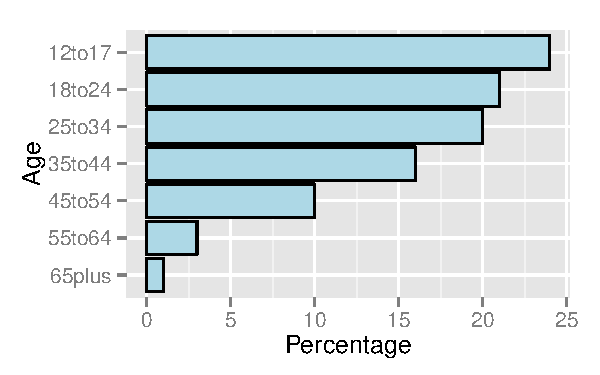
\includegraphics{figures/ex26.eps}
          \caption{Exercise 26}
        \end{figure}

        The correlation is 0.5653 so it looks like there is a mild preference
        for tall people to date each other.

      \item[27]
        \begin{parts}
          \part
            \begin{figure}[H]
              \centering
              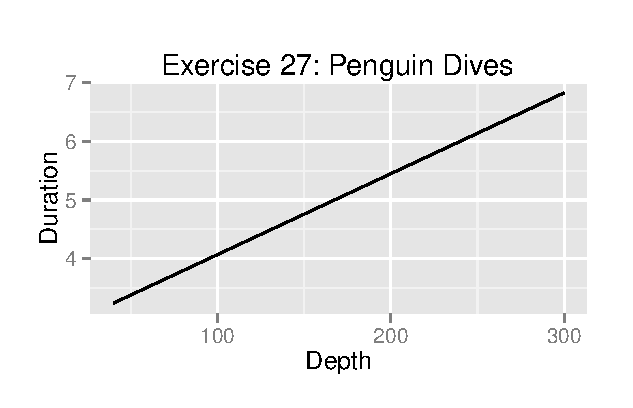
\includegraphics{figures/ex27.eps}
              \caption{Exercise 27}
            \end{figure}

          \part
            The correlation is 0.9552.  There is a strong correlation between the
            coffee price and deforestation.

          \part
            The units of the price don't matter.  Changing the currency would just
            change the labels on the y axis.

        \end{parts}

      \item[28]
        \begin{figure}[H]
          \centering
          \includegraphics{figures/ex28.eps}
          \caption{Exercise 28}
        \end{figure}

        \begin{parts}
          \part
            The correlation is -0.7485.  There is a fairly strong negative correlation 
            between the number of birds that come back and the number of new birds.

            There probably isn't any room for new birds when large numbers of returning
            birds take up all the space.

          \part
            The sparrowhawk seems to be a long-lived territorial bird.

        \end{parts}

      \item[29]
        \begin{parts}
          \part
            \begin{figure}[H]
              \centering
              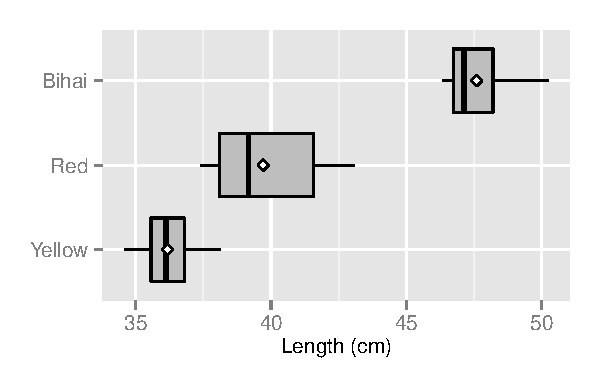
\includegraphics{figures/ex29.eps}
              \caption{Exercise 29}
            \end{figure}

          \part
            There is a strong positive correlation with one outlier at (155.2, 1.94).

          \part
            \begin{tabular}[H]{lr}
              \toprule
              with outlier    & 0.8486 \\
              without outlier & 0.7015 \\
              \bottomrule
            \end{tabular}

            The outlier has large positive z-scores for both neural activity and
            behavior, so it makes a large contribution to the total when computing
            the correlation.

        \end{parts}

      \item[31]
        \begin{figure}[H]
          \centering
          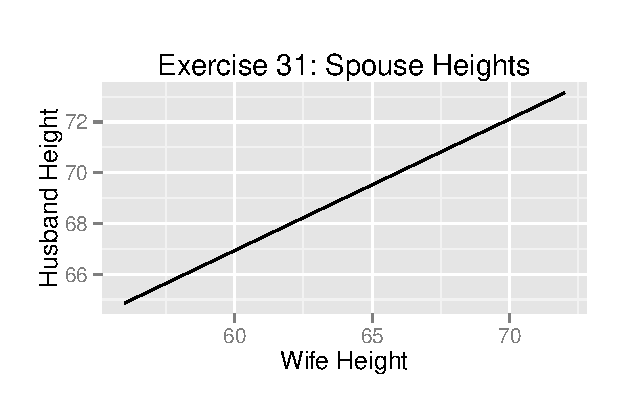
\includegraphics{figures/ex31.eps}
          \caption{Exercise 31}
        \end{figure}

        There is a strong correlation between time and icicle length.  Not surprisingly,
        if you pour water over an icicle, it gets longer over time.

        Also unsurprisingly, the more water you pour over the icicle, the faster it grows.
        Run 8903, with $\unit[29.6]{mg/s}$ grew faster than run 8905 with
        $\unit[11.9]{mg/s}$.

        Doubling the amount of water didn't double the growth rate.  Run 8903 grew only
        slightly faster than run 8905.

      \item[32]
        \begin{parts}
          
          \part
            \begin{figure}[H]
              \centering
              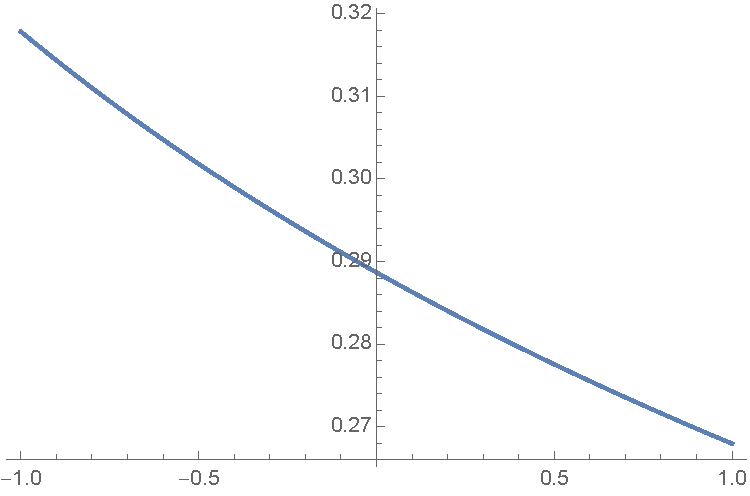
\includegraphics{figures/ex32.eps}
              \caption{Exercise 32}
            \end{figure}

          \part The pattern is vaguely linear with a weak positive correlation of 0.1349.

          \part When you add the means, you can see that the best choice is 20 plants per
          acre.

        \end{parts}

      \item[34]
        \begin{parts}
          \part Changing the units would just change the labels on the y-axis.  It
          wouldn't change the correlation.  

          \part Subtracting 6 from all the men's heights doesn't change the correlation
          either.  This is just like changing the scale.

          The correlation just indicates that women tend to date men of similar
          heights.  It doesn't say anything about whether the women (tall or not)
          tend to date men that are taller than they are.

          \part In this case the correlation would be a perfect 1.
        \end{parts}

      \item[36] This might happen if the two funds both invest in companies in the same
        industry but one fund includes primarily large companies and the other fund
        includes primarily small companies.  
        
        The large company stocks are fairly stable so they don't tend to go up and down
        much.  The small company stocks tend to move up and down more.  Both funds move
        the same direction because both small and large companies do well or badly for the
        same reasons.

        An investor which didn't want to take risks would invest in the fund which
        only moved 10\%.  He wouldn't make too much money but he also wouldn't lose
        too much money.  Another investor who didn't mind more risk might invest in
        the small company stocks.  He would have a chance to make more money, but
        that would come with a chance to lose more as well.

      \item[37]
        \begin{parts}
          \part Rachel should invest in small-cap stocks.  When her bonds plummet in
          value, her small-cap stocks are likely to only drop slightly.

          \part She should look for a fund with a negative correlation.
        \end{parts}

      \item[38]
        The report doesn't say that good researchers make bad teachers.  It just says that
        you can't draw any conclusions about teaching ability from research ability and
        vice versa.  Some excellent researchers are also excellent teachers and some
        excellent researchers are horrible teachers.

      \item[39]
        \begin{parts}
          \part You can't have a correlation between a categorical variable and a
          quantitative variable.  You need two quantitative variables.

          \part Correlations are always less than or equal to 1.

          \part Correlations don't have units.
        \end{parts}

      \item[43]
        \begin{figure}[H]
          \centering
          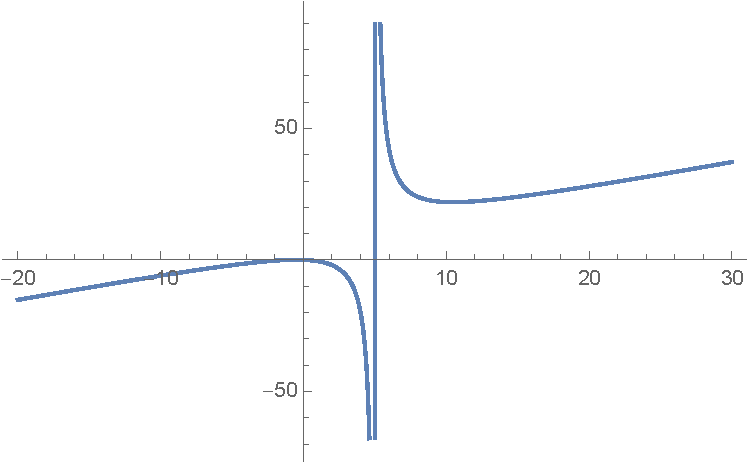
\includegraphics{figures/ex43.eps}
          \caption{Exercise 43}
        \end{figure}

        It looks like people tend to use about the same gas (not much) in the warm months,
        with or without solar panels.  People with solar panels tend to use less gas than
        people without in the cold months.

        In either case there is a strong positive correlation between cold months (high
        degree days) and gas usage.

      \item[44]
        \begin{figure}[H]
          \centering
          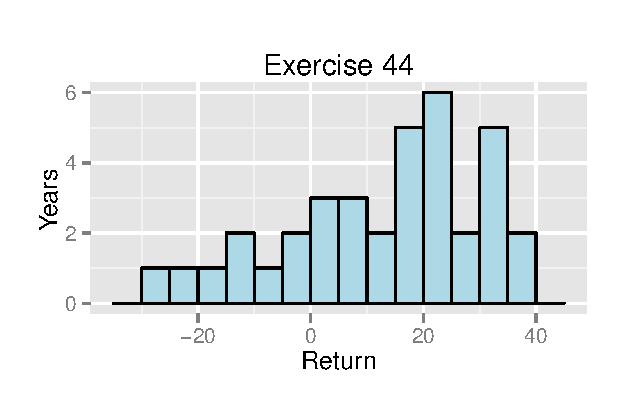
\includegraphics{figures/ex44.eps}
          \caption{Exercise 44}
        \end{figure}

        The more breeding pairs there are, the fewer pairs return each year.
    \end{description}


  \else
    \vspace{11 cm}
    \begin{quote}
      \begin{em}
        Even voting for the right is doing nothing for it. It is only expressing to men
        feebly your desire that it should prevail. 
        % A wise man will not leave the right to the mercy of chance, nor wish it to
        % prevail through the power of the majority. There is but little virtue in the
        % action of masses of men. When the majority shall at length vote for the
        % abolition of slavery, it will be because they are indifferent to slavery, or
        % because there is but little slavery left to be abolished by their vote. 
      \end{em}
    \end{quote}
    \hspace{1 cm} --Henry David Thoreau
  \fi

\end{document}

